\documentclass[border=4pt,varwidth=17cm]{standalone}
\usepackage{amsmath,amssymb,mathrsfs,mathtools}
\usepackage{tikz}
\usetikzlibrary{positioning,fit,backgrounds,arrows.meta}
\def\RR{{\mathbb R}}\def\eps{\varepsilon}\def\then{\Rightarrow}
\def\J{\mathcal{J}_L}\def\A{\mathcal{A}_{f,g}}\def\Sol{\mathcal{S}_{f,g}}
\def\limsup{\mathop{\overline{\lim}}}\def\liminf{\mathop{\underline{\lim}}}
\def\Of{{\sf (O$_f$)}}\def\Og{{\sf (O$_g$)}}
\def\Rv{{\sf (R$_{\rm v}$)}}\def\Rh{{\sf (R$_{\rm h}$)}}
\begin{document}


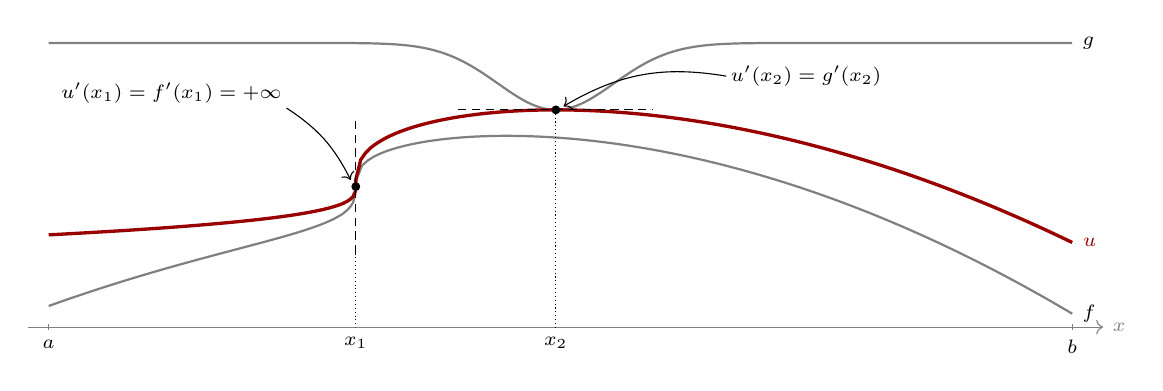
\begin{tikzpicture}[x=1.3cm, y=0.85cm, font=\scriptsize,
  declare function={C(\t)=((\t<0) ? -1 : 1)*abs(\t)^(1/3);
    F(\t)=2.1+0.8*C(\t-3)-0.07*(\t-3)^2;
    UL(\t)=2.1-0.5*abs(\t-3)^(1/3);
    UR(\t)=2.1+1.1*abs(\t-3)^(1/3)-0.06*(\t-3)^2;
    G(\t)=4.2461-exp(-((\t-4.9546)/0.8)^2);}]
  \draw[->, gray] (-0.2,0) -- (10.3,0) node[right] {$x$};
  \draw[gray] (0,0.05) -- (0,-0.05) node[below, black] {$a$};
  \draw[gray] (10,0.05) -- (10,-0.05) node[below, black] {$b$};
  % obstacles
  \draw[thick, gray, domain=0:2.999, samples=120] plot (\x, {F(\x)});
  \draw[thick, gray, domain=3.001:10, samples=120] plot (\x, {F(\x)}) node[right, black] {$f$};
  \draw[thick, gray] (2.999,{F(2.999)}) -- (3.001,{F(3.001)});
  \draw[thick, gray, domain=0:10, samples=150, smooth] plot (\x, {G(\x)}) node[right, black] {$g$};
  % solution
  \draw[very thick, red!60!black, domain=0:2.999, samples=120] plot (\x, {UL(\x)});
  \draw[very thick, red!60!black, domain=3.001:10, samples=150] plot (\x, {UR(\x)}) node[right] {$u$};
  \draw[very thick, red!60!black] (2.999,{UL(2.999)}) -- (3.001,{UR(3.001)});
  % contact with f: vertical tangent
  \fill (3,2.1) circle (1.6pt);
  \draw[densely dashed] (3,1.1) -- (3,3.1);
  \draw[densely dotted] (3,1.1) -- (3,0) node[below] {$x_1$};
  \node[align=center, fill=white, inner sep=1.5pt] (n1) at (1.2,3.5) {$u^\prime(x_1)=f^\prime(x_1)=+\infty$};
  \draw[->, thin] (n1.south east) to[bend left=15] (2.95,2.2);
  % contact with g
  \fill (4.9546,3.2461) circle (1.6pt);
  \draw[densely dashed] (4.0,3.2461) -- (5.9,3.2461);
  \draw[densely dotted] (4.9546,3.2461) -- (4.9546,0) node[below] {$x_2$};
  \node[align=center, fill=white, inner sep=1.5pt] (n2) at (7.4,3.75) {$u^\prime(x_2)=g^\prime(x_2)$};
  \draw[->, thin] (n2.west) to[bend right=20] (5.03,3.3);
\end{tikzpicture}


\end{document}
